%!TEX root = ../Bachelorseminar-RoboticSwarms.tex

In the past sections, we reviewed the most common problems found in the field of robotic swarms. 
These problems however, do overlap, because the problems found in this field often consist of multiple different problems. 
We focused on each problem, highlighting the communication methods of every solution and properties of these communication methods. 
These properties can be summarized in a Venn diagram, allowing for a compact overview of these solutions. 

	\begin{figure}[h]
		\label{venn_diagram}
		\caption{Super-awesome Venn-diagram}

		\centering

		\def\loclb{(180:2.0cm) circle (2.0cm)}
	  	\def\loclf{(0:2.0cm) circle (2.0cm)}
	  	\def\locrb{(90:2.0cm) circle (2.0cm)}
	  	\def\locrf{(270:2.0cm) circle (2.0cm)}

	    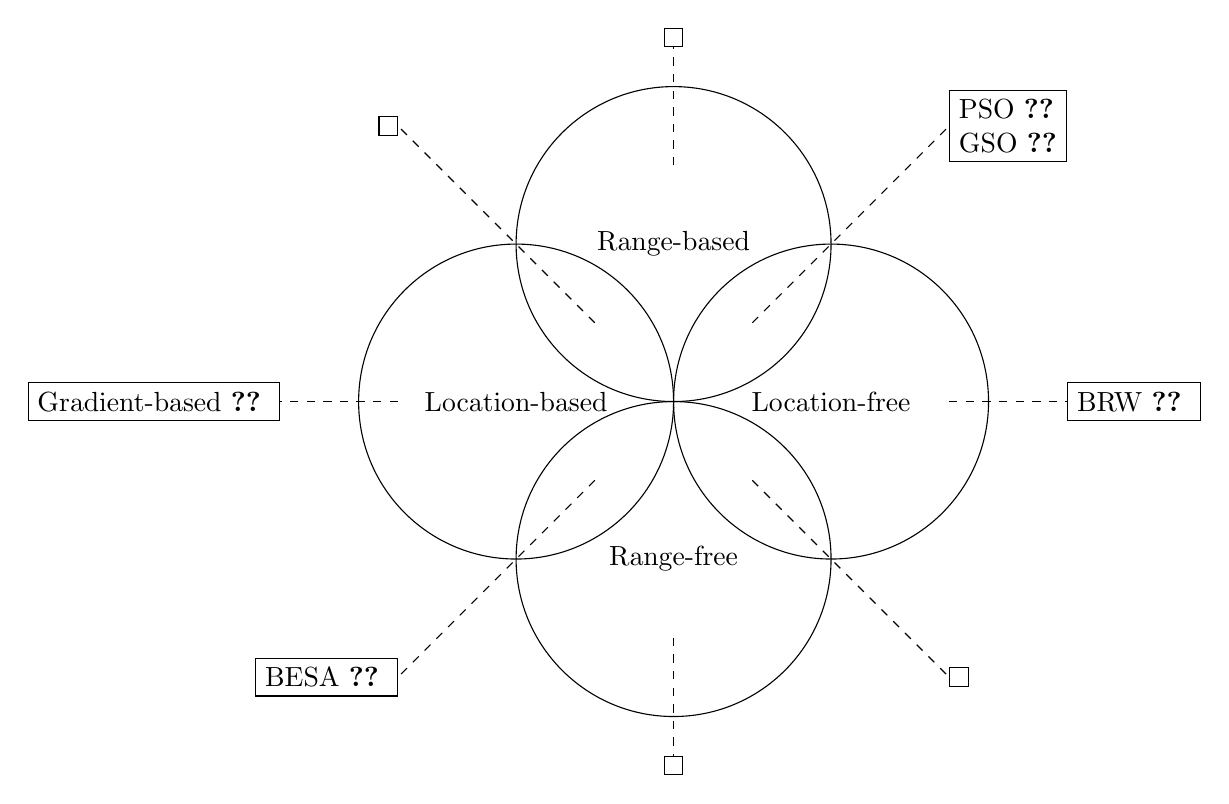
\begin{tikzpicture}
			% standard figures
			\draw \loclb node [text=black] {Location-based};
			\draw \loclf node [text=black] {Location-free};
			\draw \locrb node [text=black] {Range-based};
			\draw \locrf node [text=black] {Range-free};

			% Range-based location-free
			\draw[dashed,-] (1,1) -- (3.5,3.5) node[anchor=north west] {};
			\node[draw,align=left,anchor=west] at (3.5,3.5) {
				PSO \ref{sec:Localization}\\
				GSO \ref{sec:Localization}
			};

			% Range-free, location-free
			\draw[dashed,-] (1,-1) -- (3.5,-3.5) node[anchor=north west] {};
			\node[draw,align=left,anchor=west] at (3.5,-3.5) {

			};

			% location-free
			\draw[dashed,-] (3.5,0) -- (5,0) node[anchor=north west] {};
			\node[draw,align=left,anchor=west] at (5,0) {
				BRW \ref{sec:Localization}
			};

			% location-based
			\draw[dashed,-] (-3.5,0) -- (-5,0) node[anchor=north west] {};
			\node[draw,align=left,anchor=east] at (-5,0) {
				Gradient-based \ref{sec:Localization}
			};

			% Range-free, location-based
			\draw[dashed,-] (-1,-1) -- (-3.5,-3.5) node[anchor=north west] {};
			\node[draw,align=left,anchor=east] at (-3.5,-3.5) {
				BESA \ref{sec:Localization}
			};

			% Range-based, location-based
			\draw[dashed,-] (-1,1) -- (-3.5,3.5) node[anchor=north west] {};
			\node[draw,align=left,anchor=east] at (-3.5,3.5) {

			};

			% Range-based
			\draw[dashed,-] (0,3) -- (0,4.5) node[anchor=north west] {};
			\node[draw,align=left,anchor=south] at (0,4.5) {

			};

			% Range-free
			\draw[dashed,-] (0,-3) -- (0,-4.5) node[anchor=north west] {};
			\node[draw,align=left,anchor=north] at (0,-4.5) {
			
			};
		\end{tikzpicture}
    \end{figure}

We see that most solutions are range-based and location-based. 
In practice, these solutions are not the most desirable solutions, because of two reasons. 
The first reason is scalability. 
Because when an algorithm is location-based and range-based, the robots used in the swarm have to be more advanced to correctly handle complex information. 
This also introduces a lot of overhead, decreasing communication speed when the robotic swarm increases in size. 
The second reason is that algorithms that are location-based can often not be used in dynamic locations, especially in algorithms where the operating environment has to be defined beforehand. 
